Encuentra el valor de $x$ en el triángulo de la figura \ref{fig:lados_pitagoras_08}.

\begin{minipage}[t][][t]{0.35\textwidth}
    \begin{figure}[H]
        \centering
        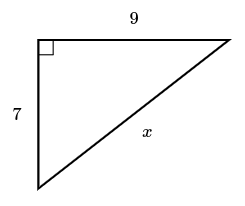
\includegraphics[width=0.9\linewidth]{../images/lados_pitagoras_08.png}
        \caption{}
        \label{fig:lados_pitagoras_08}
    \end{figure}
\end{minipage}\hfill
\begin{minipage}[t][][t]{0.6\textwidth}
    \begin{solutionbox}{9cm}
        \begin{minipage}{0.4\textwidth}
            \begin{figure}[H]
                \centering
                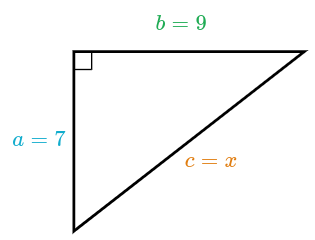
\includegraphics[width=0.9\linewidth]{../images/lados_pitagoras_08a.png}
                \caption{}
                \label{fig:lados_pitagoras_08a}
            \end{figure}
        \end{minipage}\hfill
        \begin{minipage}{0.55\textwidth}
            Tenemos un triángulo rectángulo, por lo que podemos usar el teorema de Pitágoras.
            La ecuación del teorema es:
            \[{\color{orange}c}^2={\color{cyan}a}^2+{\color{LimeGreen}b}^2\]
            donde $a$ y $b$ son las longitudes de los catetos, y $c$ es la longitud de la hipotenusa.
            Etiquetemos la Figura del problema con $a$, $b$ y $c$ (ver Figura \ref{fig:lados_pitagoras_08a}).
            Observa que $a$ y $b$ pueden intercambiarse, pues son catetos.
        \end{minipage}
        \begin{align*}
            {\color{cyan}a}^2+{\color{LimeGreen}b}^2  ={\color{orange}c}^2 & \text{\quad El teorema de Pitágoras}                          \\
            {\color{cyan}7}^2+{\color{LimeGreen}9}^2  ={\color{orange}x}^2 & \text{\quad Sustituye las longitudes}                         \\
            49+81   =x^2                                                   & \text{\quad Evalua los cuadrados conocidos}                   \\
            130=x^2                                                        & \text{\quad Sumando }                                         \\
            \sqrt{130}=x                                                   & \text{\quad Calculando la raíz en ambos lados de la ecuación} \\
        \end{align*}
    \end{solutionbox}
\end{minipage}
